\section*{\fs{12}Zapytanie z użyciem LEFT Join}
\par{
\fs{12}
\subsection*{\fs{12} Ilość kobiet przyjętych na oddział położniczy}

\listsinglespacing{
\fs{12}
\begin{lstlisting}[frame=single,language=SQL,]
Select count(*) as "Ilość kobiet" from Pobyt 
inner join 
(Select id_oddziału,nazwa from Oddział where id_oddziału=13) as O 
ON O.id_oddziału=Pobyt.oddział
left join lekarstwa_pobyt as LP on LP.id_lekarstwa=Pobyt.lekarstwa
left join Pacjent as P on P.pesel=Pobyt.pesel

\end{lstlisting}
\begin{figure}[h!]
    \centering
   \scalebox{.85}{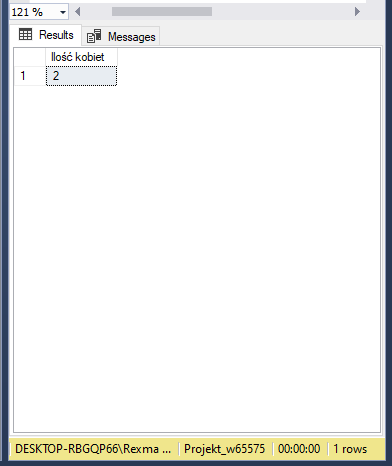
\includegraphics{Images/Zadanie3/P3/Z11a.png}}
    \caption{Wynik Zapytania}
    \label{fig:my_label}
\end{figure}
}
}
\begin{figure}[h!]
    \centering
   \scalebox{.60}{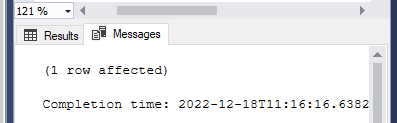
\includegraphics{Images/Zadanie3/P3/Z11b.png}}
    \caption{Wynik Zapytania}
    \label{fig:my_label}
\end{figure}

\newpage
\clearpage

\subsection*{\fs{12} Ilość badań przerowadzonych przez lekarza Owena Gregorego }

\listsinglespacing{
\fs{12}
\begin{lstlisting}[frame=single,language=SQL,]
Select nazwa from Badania
left join Pracownicy
on Pracownicy.id_pracownika=Badania.lekarz
where lekarz ='88'

\end{lstlisting}
\begin{figure}[h!]
    \centering
   \scalebox{.85}{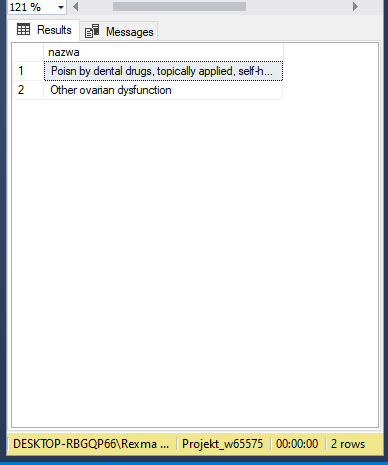
\includegraphics{Images/Zadanie3/P3/Z12a.png}}
    \caption{Wynik Zapytania}
    \label{fig:my_label}
\end{figure}
}
\begin{figure}[h!]
    \centering
   \scalebox{.85}{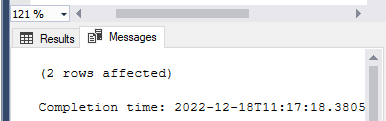
\includegraphics{Images/Zadanie3/P3/Z12b.png}}
    \caption{Wynik Zapytania}
    \label{fig:my_label}
\end{figure}
\newpage
\subsection*{\fs{12} Pacjenci i ich adresy }

\listsinglespacing{
\fs{12}
\begin{lstlisting}[frame=single,language=SQL,]
Select CONCAT(Imie,' ',nazwisko) as Pacjent, 
CONCAT(miasto, ' ',ulica, ' ' , nr_budynku , ' ',nr_mieszkania) 
as Adres  from Pacjent 
left join Adresy
on Adresy.id_adres=Pacjent.id_adres

\end{lstlisting}
\begin{figure}[h!]
    \centering
   \scalebox{.85}{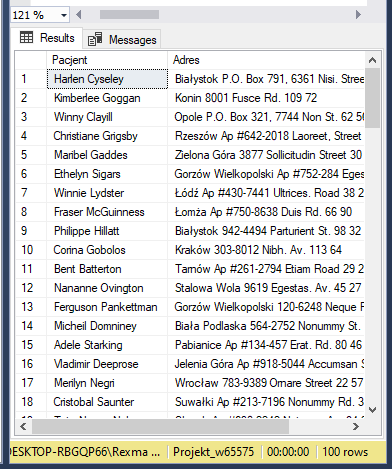
\includegraphics{Images/Zadanie3/P3/Z13a.png}}
    \caption{Wynik Zapytania}
    \label{fig:my_label}
\end{figure}
}
\begin{figure}[h!]
    \centering
   \scalebox{.60}{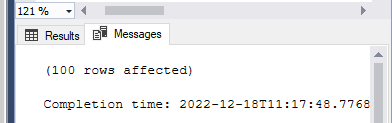
\includegraphics{Images/Zadanie3/P3/Z13b.png}}
    \caption{Wynik Zapytania}
    \label{fig:my_label}
\end{figure}
\newpage
\subsection*{\fs{12} Ilosc osób na danych stanowiskach }


\listsinglespacing{
\fs{12}
\begin{lstlisting}[frame=single,language=SQL,]
Select COUNT(*) as [ilosc],S.nazwa  from Pracownicy
left join Stanowisko as S
on Pracownicy.stanowisko=S.id_stanowiska
group by S.nazwa
having count(stanowisko)>=1
order by [ilosc]

\end{lstlisting}
\begin{figure}[h!]
    \centering
   \scalebox{.85}{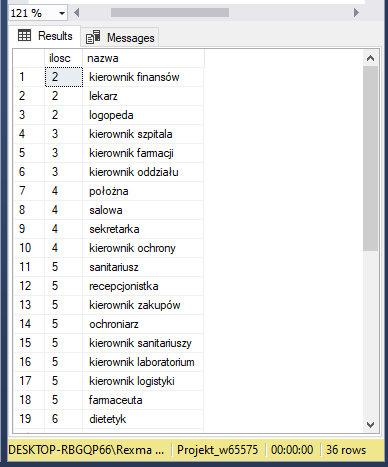
\includegraphics{Images/Zadanie3/P3/Z14a.png}}
    \caption{Wynik Zapytania}
    \label{fig:my_label}
\end{figure}
}
\begin{figure}[h!]
    \centering
   \scalebox{.60}{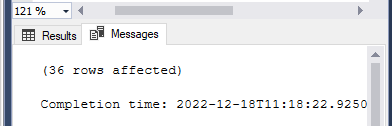
\includegraphics{Images/Zadanie3/P3/Z14b.png}}
    \caption{Wynik Zapytania}
    \label{fig:my_label}
\end{figure}\newpage

\newpage
\subsection*{\fs{12} Wizyty }


\listsinglespacing{
\fs{12}
\begin{lstlisting}[frame=single,language=SQL,]
Select W.data,W.opis,
CONCAT(W.pesel,' ',Pa.imie,' ',Pa.nazwisko) as Pacjent,
W.recepta,CONCAT(P.imie,' ',P.nazwisko) as Lekarz
from Wizyty as W
left join Recepta as R
on R.id_recepty=W.recepta
left join Pracownicy as P
on P.id_pracownika=R.id_recepty
left join Pacjent as Pa
on Pa.pesel=W.pesel
order by data

\end{lstlisting}
\begin{figure}[h!]
    \centering
   \scalebox{.85}{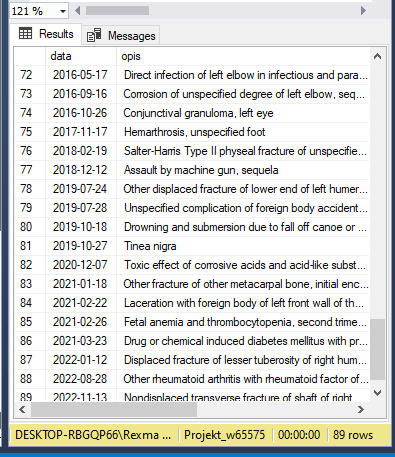
\includegraphics{Images/Zadanie3/P3/Z15a.png}}
    \caption{Wynik Zapytania}
    \label{fig:my_label}
\end{figure}
}
\begin{figure}[h!]
    \centering
   \scalebox{.60}{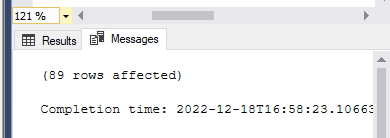
\includegraphics{Images/Zadanie3/P3/Z15b.png}}
    \caption{Wynik Zapytania}
    \label{fig:my_label}
\end{figure}\newpage